\documentclass[11pt]{article}
%\documentclass[preprint, 10pt]{elsarticle}

% PACKAGES
\usepackage{graphicx, amsmath, amssymb, amsfonts, mathtools, mathrsfs, color}
\usepackage{comment, enumerate, tabularx}
\usepackage{natbib, hyperref, url}
\usepackage[margin=1in]{geometry}
%\usepackage[justification=RaggedRight]{caption}

%----------------------------------------------------------------------------%
%% LATEX DEFINITIONS
%----------------------------------------------------------------------------%
% Basic editing
\newcommand{\tocite}{{\color{blue}(to cite)}}
\newcommand{\vsp}[1]{\vspace{#1 pc} \noindent}
\newcommand{\np}{\newpage \noindent}
\newcommand{\nick}[1]{{\color{red} #1}}
% Derivatives
\newcommand{\pd}[2]    { \frac{\partial #1} {\partial #2} }
\newcommand{\ppd}[2]  { \frac{\partial^2 #1}{{\partial #2}^2} }
\newcommand{\pdi}[2] { {\partial_#2} #1 }
\newcommand{\td}[2] { \frac{d #1} { d #2 } }
\newcommand{\grad}{\nabla}
\newcommand {\Lap} {\grad^2}
% Vectors and operators
\newcommand{\bvec}[1]{\ensuremath{\boldsymbol{#1}}}
\newcommand{\abs}[1]{\left| #1 \right|}
\newcommand{\norm}[1]{\left\| #1 \right\|}
\newcommand{\mean}[1]{\left< #1 \right>}
\newcommand{\eps}{\varepsilon}
\newcommand{\dx}{\, dx}
\newcommand{\CC}{{\mathbb{C}}}
% Basic physical parameters and scales
\newcommand{\freqp}{f_p}
\newcommand{\etastd}{\eta_{\text std}}
% Parameters that change crossing the ADC
\newcommand{\depth}{d}
\newcommand{\dup}{\depth_{-}}
\newcommand{\ddn}{\depth_{+}}
\newcommand{\dupdn}{\depth_{\pm}}
\newcommand{\lam}{\lambda}
\newcommand{\lamup}{\lam_{-}}
\newcommand{\lamdn}{\lam_{+}}
\newcommand{\lamupdn}{\lam_{\pm}}
\newcommand{\lamfac}{N}
\newcommand{\drat}{\mathcal{D}}
\newcommand{\dratdn}{\drat_+}
\newcommand{\dratupdn}{\drat_{\pm}}
% Statistical quantities
\newcommand{\En}{\mathcal{E}}
\newcommand{\Mo}{\mathcal{M}}
\newcommand{\skw}{\text{skew}}
\newcommand{\skwdn}{\skw_+}
\newcommand{\var}{\text{var}}
\newcommand{\varup}{\var_-}
\newcommand{\vardn}{\var_+}
\newcommand{\kurt}{\text{kurt}}
\newcommand{\std}{\text{std}}
% Dimensionless parameters
\newcommand{\ampscale}{\mathcal{A}}
\newcommand{\lengthscale}{\mathcal{L}}
\newcommand{\timescale}{\mathcal{T}}
\newcommand{\epsup}{\eps_0}
\newcommand{\delup}{\delta_0}
% Hamiltonian stuff
\newcommand{\uhat}{\hat{u}}
\newcommand{\sympJ}{\mathcal{J}}
\newcommand{\vard}[2]{\frac{\delta #1}{\delta #2}}
\newcommand{\Ham}{\mathcal{H}}
\newcommand{\Hup}{\Ham^{-}}
\newcommand{\Hdn}{\Ham^{+}}
\newcommand{\Hupdn}{\Ham^{\pm}}
\newcommand{\Hthree}{\Ham_{3}}
\newcommand{\Htwo}{\Ham_{2}}
%\newcommand{\Fcnl}{\mathcal{F}}
% Truncated stuff
\newcommand{\Proj}{\mathcal{P}_{\Lambda}}
\newcommand{\uL}{u_{\Lambda}}
\newcommand{\HLupdn}{\Ham_{\Lambda}^{\pm}}
\newcommand{\SympL}{\sympJ_{\Lambda}}
\newcommand{\uup}{u_{-}}
\newcommand{\udn}{u_{+}}
\newcommand{\uupdn}{u_{\pm}}
% Gibbs and theta
\newcommand{\Gibbs}{\mathcal{G}}
\newcommand{\Gup}{\Gibbs^{-}}
\newcommand{\Gdn}{\Gibbs^{+}}
\newcommand{\Gupdn}{\Gibbs^{\pm}}
\newcommand{\thup}{\theta^{-}}
\newcommand{\thdn}{\theta^{+}}
\newcommand{\thupdn}{\theta^{\pm}}
\newcommand{\meanup}[1]{\mean{#1}_{-}}
\newcommand{\meandn}[1]{\mean{#1}_{+}}
\newcommand{\meanupdn}[1]{\mean{#1}_{\pm}}
\newcommand{\Gz}{\Gibbs_0}
\newcommand{\meanz}[1]{\mean{#1}_0}
% Stuff
\newcommand{\tavg}[1]{\overline{#1}}
\newcommand{\transf}{\mathcal{F}}
\newcommand{\Nsamp}{N_s}
\newcommand{\sumsamp}{\sum_{i=1}^{\Nsamp}}

% Experiments
\newcommand{\omavg}{\omega_0}
\newcommand{\omsig}{\sigma_{\omega}}
\newcommand{\Dphi}{\Delta \phi}

%----------------------------------------------------------------------------%

%----------------------------------------------%
%% TITLE
%----------------------------------------------%
\begin{document}

\title{Anomalous waves triggered by abrupt depth changes: experiments and truncated KdV theory}

%experimental measurements and deterministic-statistical truncated KdV theory
% ORIGINAL: The truncated KdV framework for modeling anomalous waves induced by abrupt depth changes
% Words: triggered, induced, generated, sparked

\author{
M.~N.~J.~Moore\thanks{Florida State University}, 
C.~Tyler Bolles\thanks{University of Michigan},
Andrew J.~Majda\thanks{Courant Institute of Mathematical Sciences}, 
Di Qi\thanks{Courant Institute of Mathematical Sciences} }
\maketitle

\begin{abstract} 
Recent laboratory experiments revealed the emergence of anomalous statistics in a randomized surface waves upon encountering an abrupt depth change (ADC) in the bottom topography (Bolles et al. PRF 2019). Majda et al.~2019 established a theoretical foundation, based on analysis of the truncated KdV (TKdV) system, that successfully captures several key qualitative features of the experiments including the robust emergence of anomalous statistics. The framework exploits the Hamiltonian structure of TKdV to construct invariant measures that are statistical matched at the ADC, and is corroborated by simulations of the deterministic dynamics. 
%
Here we present a more comprehensive treatment of these parallel experimental and modeling efforts, with emphasis on the link between the two. We present an assortment of new experimental measurements and carefully compare them to model predictions. We establish a more precise link between experimental and model parameters, so that the invariant measure underlying the model can be calibrated to the specific conditions present in experiments. The model predicts a peculiar relationship between surface-displacement skewness and surface-slope variance, which is confirmed in spectacular fashion by direct experimental measurements.
\end{abstract}


%----------------------------------------------------------%
% Intro
%----------------------------------------------------------%
\section{Introduction}

Rogue waves are abnormally large surface waves, defined by oceanographers as those that exceed twice the significant wave height \citep{muller2005rogue, ying2011linear}. Though such waves were once dismissed as myth, they have now been recorded in oceans across the globe and pose a recognized threat to seagoing vessels and naval structures. Rogue waves, also variously known as freak or anomalous waves, have been observed both in deep and shallow water, and can be triggered by a variety of mechanisms, including anomalous wind-forcing \citep{kharif2008influence, toffoli2017wind}, opposing currents \citep{garrett2009rogue, onorato2011triggering},
focusing due to variable bathymetry \citep{heller2008refraction, white1998chance}, 
and the Benjamin-Feir deep-water modulational instability \citep{benjamin1967disintegration, viotti2013emergence, cousins2015unsteady, farazmand2017reduced}.
The common tie between these mechanisms is their ability to generate non-normal statistics in the surface displacement; when governed by Gaussian statistics, the likelihood of a rogue wave is extremely low, but these rare events occur much more frequently when surface statistics deviate from Gaussian. In this way, it makes sense to approach anomalous waves from the broader perspective of turbulent dynamical systems \cite{sapsis2013a, sapsis2013b, sapsis2013blending, chen2016filtering, majda2016introduction, macedo2017universality, MajdaQiSIAM2018, blonigan2019extreme, guth2019machine}.

A recent series of laboratory \cite{bolles2019} and numerical investigations \cite{viotti2014} have demonstrated the emergence of anomalous wave statistics from abrupt variations in bottom topography. Since topographical variations are strictly one-dimensional, these studies can be viewed as offering a bare minimum set of conditions capable of generating anomalous wave statistics. In particular, the more complex mechanism of focusing by 2D bottom topography absent. The studies thus offer a paradigm system, with emergent anomalous statistical properties similar to that seen in more complex systems, but in a tractable context that is amenable to analysis.

Our particular focus is the laboratory experiments of Bolles et al.~\cite{bolles2019}, who demonstrated the emergence of anomalous statistics from a randomized wave-field encountering an abrupt depth change (ADC). In these experiments, the incoming wave-field is generated with nearly Gaussian statistics, and a plexiglass step placed near the middle of the tank creates the depth change. Upon passing into the shallower region, the wave distribution skews strongly towards positive displacement, with deviation from Gaussian being most pronounced a short distance downstream of the ADC. Inspired by these experimental observations, Majda et al.~\cite{majda2019} developed a theoretical framework that accurately captures several key aspects of the anomalous behavior. The theory is based on deterministic and statistical analysis of the truncated Korteweg–de Vries (TKdV) equations, and uses a combination of computational, statistical, and analytical tools. In subsequent work, Majda and Qi \cite{majdaqi2019} analyzed more severely truncated systems that were shown to exhibit many of the same anomalous properties while enjoying a more tractable, lower-dimensional structure.

The purpose of the present manuscript is to provide a more comprehensive treatment of the {\em combined} experimental and theoretical efforts of Bolles et al~\cite{bolles2019} and Majda et al.~\cite{majda2019, majdaqi2019}. Special emphasis is placed on the synergy between experiment and theory -- a cooperative strategy with a proven record of success \cite{camassa2012stratified, ristroph2012, ganedi2018equilibrium}. We present an assortment of previously unpublished experimental data, for example on surface slope statistics and autocorrelation, which motivates further examination and refinement of the theory. Likewise, novel theoretical predictions have inspired us to perform additional experimental measurements, especially as it pertains to a peculiar relationship between surface-displacement skewness and surface-slope variance that is predicted by the theory. Comparison with the new measurements further confirms the predictive power of the framework developed by Majda et al.~\cite{majda2019}. In addition, we provide a more thorough treatment of the link between experimental and model parameters to facilitate comparison between the two. In particular, we flesh out details of non-dimensionalization, which were only briefly addressed in prior work for the sake of brevity.

% NOTES
% Words: conjunction, combination, close cooperation; elucidate.
% New data: slopes, autocorrelation, depth ratio varied.


%----------------------------------------------------------%
% Experiments
%----------------------------------------------------------%
\section{The experiments}
\label{experiments}

	As diagrammed in Fig.~\ref{ExpDiagStats}(a), the experiments consist of a long, narrow wave tank (6 m long x 20 cm wide x 30 cm high), with waves generated by plexiglass paddle at one end \cite{bolles2019}. The waves propagate through the tank and, roughly midway through, pass over an abrupt depth change (ADC) created by a plexiglass step. The waves continue to propagate through the shallower depth until reaching the far end of the tank, at which point their energy is dissipated by a horse-hair dampener. Since the dampener minimizes backscatter, the waves in this experiment propagate primarily in one direction, from left to right in Fig.~\ref{ExpDiagStats}(a). 

The pivoting motion of the paddle is driven by a 5-phase stepper motor. To generate a randomized wave field, the paddle angle $\phi$ is specified by a psuedo-random signal
\begin{align}
\label{PaddleAngle}
& \phi(t) = \phi_0 + \Dphi \sum_{n=1}^N a_n \cos(\omega_n t+\delta_n) \, , \\
\label{anEq}
& a_n = \sqrt{\frac{2 \Delta \omega}{\pi^{1/2} \omsig}} \, 
\exp \left( -\frac{(\omega_n - \omavg)^2}{2 \omsig^2} \right) \, ,
\end{align}
The angular frequencies are evenly spaced $\omega_n = n  \Delta \omega$ with step size $ \Delta \omega = (\omavg+4 \omsig)/N$, where $\omavg$ and $\omsig$ represent the mean and the bandwidth of $\omega$ respectively. As in prior work, all experiments reported here use the values $\omavg = \omsig = 12.5$ rad/s, corresponding to a peak forcing frequency of 2 Hz and bandwidth of 2 Hz. The phases $\delta_n$ are uniformly distributed random variables, which results in a randomized wave train. The standard deviation of the paddle angle, $\Dphi$, controls the amplitude overall amplitude of the waves. In a single experiment $\Dphi$ is fixed, and we will present a series of experiments with $\Dphi$ varied systematically. 

% Figure: Experimental Diagram and Histograms
%^^^^^^^^^^^^^^^^^^^^^^^^^^^^^^%
\begin{figure}%[!ht]
\begin{center}
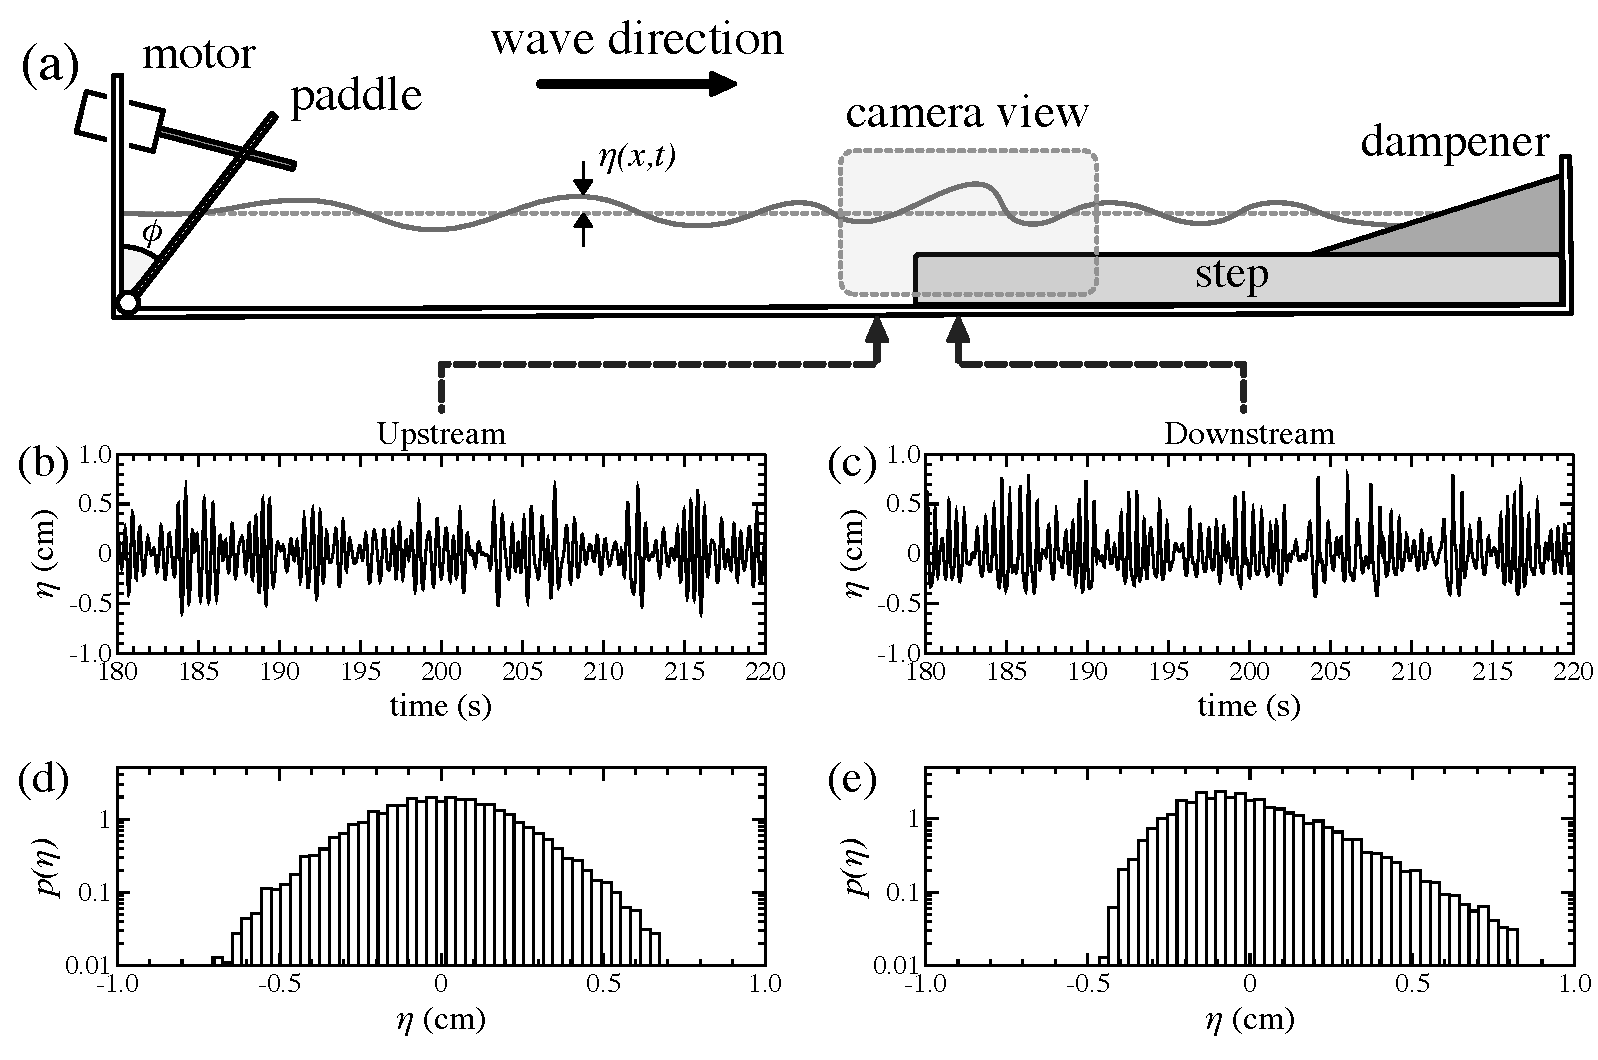
\includegraphics[width = 0.80 \linewidth]{Figs/ExpDiagStats.pdf}
\caption{
(a) Experimental schematic. 
(b)--(c) Surface displacement measured at a representative upstream and downstream locations. (d)--(e) Corresponding histograms. Figure adapted from \cite{bolles2019}.}
\label{ExpDiagStats}
\end{center}
\end{figure}
%^^^^^^^^^^^^^^^^^^^^^^^^^^^^^^%
% Data from column 5 in MasterTimeSeries, Delta theta = 1.38 degrees, which is in between runs 5 and 6.
 
	The free surface is illuminated by light-emitting diodes and is imaged from the sideview with a Nikon D3300 at 60 frames per second. The illumination technique, coupled with high pixel count of the camera, allows surface displacements to be resolved with accuracy better than 1/3 millimeter. Furthermore, these optical measurements permit extraction of wave statistics {\em continuously} in space, rather than at a few discrete locations, which is crucial for identifying regions of anomalous wave activity. Further details of the experimental setup can be found in \cite{bolles2019}.

	Example measurements of free-surface displacements $\eta$ are shown in Figs.~\ref{ExpDiagStats}(b)--(c). These measurements are extracted from the images at two representative locations: one a short distance (9 cm) upstream of the ADC and the other a short distance (15 cm) downstream. Both signals exhibit a combination of periodic and random behavior, with the dominant oscillations corresponding to the peak forcing frequency of 2 Hz. The nature of the random fluctuations is revealed by the corresponding histograms shown in Fig.~\ref{ExpDiagStats}(d)--(e). The upstream measurements are symmetrically distributed about the mean, $\eta = 0$. In fact, Bolles et al.~found that these measurements follow a Gaussian distribution closely \cite{bolles2019}. The downstream measurements, however, skew strongly towards positive displacement, $\eta > 0$. Bolles et al.~found these measurements to be well described by a mean-zero gamma distribution \cite{bolles2019}. The slower decay rate of this downstream distribution indicates an elevated level of extreme surface displacement, i.e.~rogue waves. Bolles et al.~estimated that a rogue wave can be up to 65 times more likely in these experiments than if displacements were Gaussian \cite{bolles2019}. 

% Figure: Experimental Spatial Statistics
%^^^^^^^^^^^^^^^^^^^^^^^^^^^^^^%
\begin{figure}%[!ht]
\begin{center}
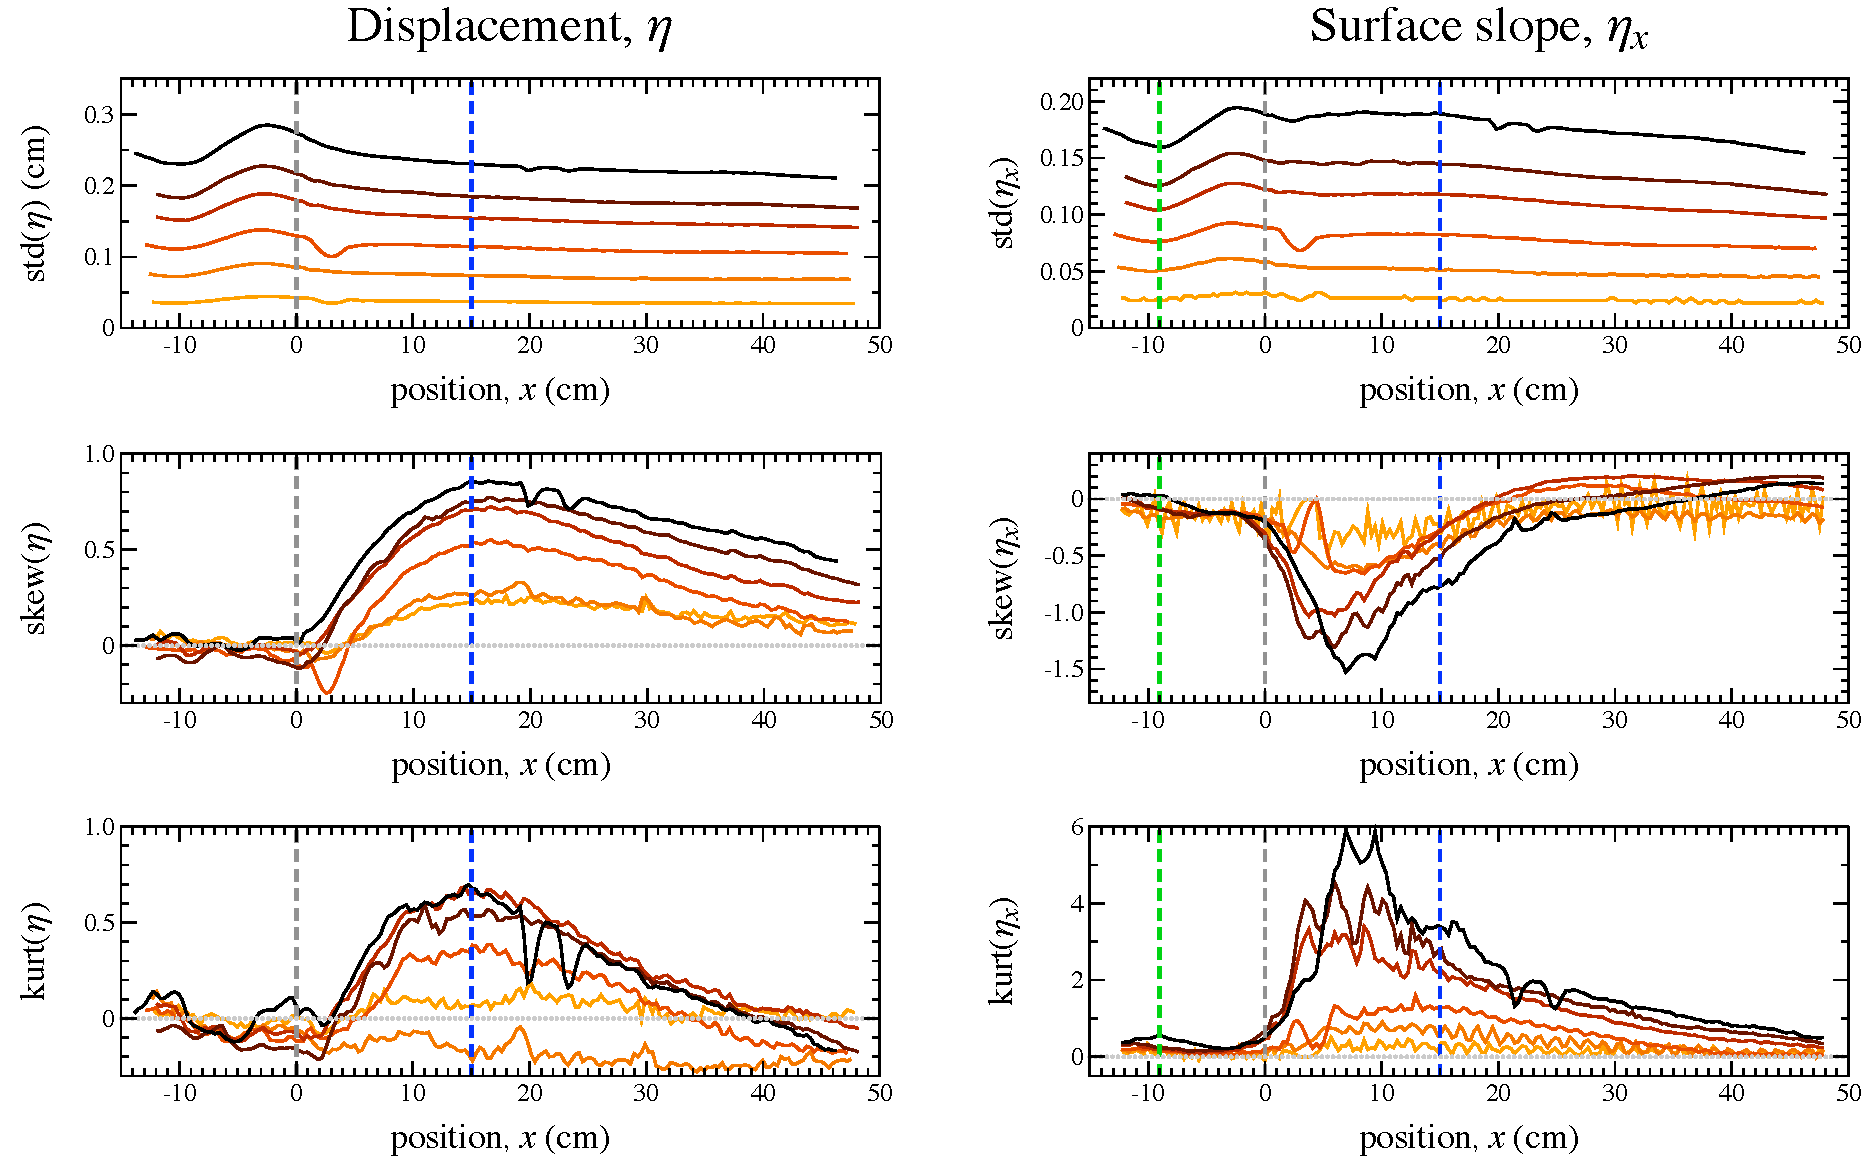
\includegraphics[width = 0.85 \linewidth]{Figs/ExpSpatialStats.pdf}
\caption{Wave statistics as they vary in space for several different experiments of different driving amplitudes (see legend). (a)--(c) Standard deviation, skewness, and kurtosis of the surface displacement $\eta$. (d)--(f) The same for surface slope $\eta_x$. A reference wave amplitude is set by $\etastd$ which does not vary significantly crossing the ADC. Skewness and kurtosis of $\eta$, however, show a strong response to the ADC. The surface slope measurements are negatively skewed and also show a large kurtosis downstream of the ADC. }
\label{ExpSpatialStats}
\end{center}
\end{figure}
 %^^^^^^^^^^^^^^^^^^^^^^^^^^^^^^%
 
	The paddle amplitude in Fig.~\ref{ExpDiagStats} is $\Dphi = 1.38^{\circ}$, and this value was varied systematically in the range $\Dphi = 0.125^{\circ}$--$2^{\circ}$ to probe the different regimes of wave behavior, from linear to strongly nonlinear waves. Figure \ref{ExpSpatialStats} shows long-time statistics of both surface displacement $\eta$ and the surface slope $\eta_x$ as they vary in space for six different driving amplitudes (see legend). We will only be examining statistics of mean-zero quantities in this paper, and so, for an arbitrary mean-zero quantity $q$, we have the following definitions
\begin{align}
%& \var(q) = \mean{q^2}		&&\mbox{\em variance} \\
& \std(q) = q_{std}= \sqrt{\mean{q^2}}
&&\mbox{\em standard deviation} \\
& \skw(q) = {\mean{q^3}} / {q_{std}^3}	
&&\mbox{\em skewness} \\
& \kurt(q) = {\mean{q^4}} / {q_{std}^4} - 3
&&\mbox{\em (excess) kurtosis}
\end{align}
where $\mean{}$ indicates a mean (here a long-time mean). Hereafter, we will simply refer to the excess kurtosis as kurtosis.

	Figure \ref{ExpSpatialStats} shows how these statistics vary in the vicinity of the ADC, located at $x = 0$, for both displacement and slope. First, the standard deviation of displacement, $\etastd$, gives the coarsest possible estimate for the amplitude of waves. Figure \ref{ExpSpatialStats}(a) shows that while $\etastd$ increases with driving amplitude, it remains relatively uniform in space for each individual experiment, indicating that the overall amplitude of the wave train is not significantly altered by the presence of the ADC. In experiments with sufficiently high driving amplitude, though, the skewness and kurtosis (b)--(c) respond strongly to the ADC. In these experiments, both the skewness and kurtosis are relatively small upstream of the ADC, indicating nearly Gaussian statistics, but then increase dramatically downstream and reach a peak near $x = 15$ cm. Remarkably, the location of the peak is the same for skewness and kurtosis and appears insensitive to driving amplitude. The maximum values of skewness and kurtosis (roughly 0.9 and 0.7 respectively) seen in the figure indicate a significant departure from Gaussian statistics, as is constant with the histogram in Fig.~\ref{ExpDiagStats}(e). Bolles et al.~found that, once a threshold driving amplitude is exceeded (roughly $\Dphi = 0.5^{\circ}$), the displacement statistics in this anomalous region are robustly described by the gamma distribution. We note that we have gathered data for 15 different driving amplitudes, but only display 6 in Fig.~\ref{ExpSpatialStats} to avoid clutter. 

	To complement the displacement statistics, we report here statistics for the surface slope $\eta_x$ in the right column of Fig.~\ref{ExpSpatialStats}. Our attention to slope statistics was motivated by new theoretical developments by Majda et al.~\cite{majda2019} and will be expanded upon in later sections. We extract the surface slope by numerical differentiating images of the free surface using Savitzky-Golay smoothing filters. This ability to extract surface slope is another advantage of our optical measurements over the more commonly used technique of placing a set of discrete wave probes in the tank. As seen in Fig.~\ref{ExpSpatialStats}(a) the standard deviation of slope behaves similar to displacement: $\std(\eta_x)$ increases with driving amplitude, but remains nearly uniform in space for each individual experiment and is not affected by the ADC. The higher-order moments, however, once again respond strongly to the ADC if the driving amplitude is sufficiently high. The skewness of slope becomes highly negative and reaches a minimum near $x = 8$ cm, which is downstream of the ADC but upstream of the position where the displacement statistics peak. The kurtosis of $\eta_x$ reaches a peak at nearly the same location as skewness. We note that the large {\em negative} skewness of $\eta_x$ indicates a bias towards negative slope, which is consistent with a right-moving wave of steep leading surface and shallower trailing surface, i.e.~a wave that is near overturning.

	Bolles et al.~systematically explored the effect of varying the driving amplitude on the anomalous statistics for a fixed depth ratio. Here, we further explore the effect of driving amplitude, especially in conjunction with theoretical developments, and we also report experiments in which the depth ratio was varied. To have a simple baseline for comparison against theory, we refer to the data from Fig.~\ref{ExpDiagStats} as the {\em reference} experiments. In these experiments, the driving amplitude is $\Dphi = 1.38^{\circ}$ (intermediate between the two largest amplitudes shown in Fig.~\ref{ExpSpatialStats}), the upstream depth is $\dup = 12.5$ cm, and the downstream depth is $\ddn = 3$ cm, giving a depth ratio of $\dratdn = \ddn/\dup= 0.24$. From the data represented in Fig.~\ref{ExpSpatialStats}, we extract a characteristic wave amplitude for the representative experiments of $\etastd = 0.21$ cm, which will be important for setting dimensionless parameters that enter the theory. Table \ref{paramtable} lists the range of experimental parameters along with these representative values, as well as values of dimensionless parameters that will be introduced later.
% NOTE: Maybe modify slightly the last paragraph if it does not seem to fit next time I read it.

% Table
%^^^^^^^^^^^^^^^^^^^^^^^^^^^^^^%
\begin{table}[h]%[htbp]
\begin{center}
\caption{Table of parameters}
\label{paramtable}
\begin{tabular}{l l l l}
%\hline \multicolumn{3} { c }{Parameters that are constant in a single experiment} \\
\hline Description & Notation & Experimental range & `Representative' values \\
\hline
Peak forcing frequency	& $f_p$					& 2 Hz 		& 2 Hz \\
Characteristic amplitude	& $\etastd$				& 0.03--0.3 cm	& 0.21 cm \\
Upstream depth		& $\dup$					& 12.5 cm 	& 12.5 cm \\
Downstream depth		& $\ddn$					& 2.2--5.3 cm	& 3 cm \\
Upstream wavelength	& $\lamup = \sqrt{g \dup}/f_p$	& 55 cm 		& 55 cm \\
Downstream wavelength	& $\lamdn = \sqrt{g \ddn}/f_p$	& 23--36 cm	& 27 cm \\
%
Amplitude-to-depth ratio	& $\epsup = \etastd / \dup$	&0.0024--0.024	& 0.017 \\
Depth-to-wavelength ratio	& $\delup = \dup / \lamup$	& 0.23		& 0.23 \\
Depth ratio			& $\dratdn = \ddn/\dup$		& 0.18--0.42	& 0.24 \\
\end{tabular}
\end{center}
\end{table}
 %^^^^^^^^^^^^^^^^^^^^^^^^^^^^^^%


%----------------------------------------------------------%
% Theory
%----------------------------------------------------------%
\section{Theoretical framework}

We now introduce the theoretical framework that will be used to understand and quantify the experimental observations. This framework is based on a Galerkin truncation of the variable-depth Korteweg–de Vries (KdV) equation. The KdV equation is a commonly excepted model for describing the propagation of unidirectional, shallow-water waves, and it accounts for weak nonlinearity and weak dispersion over long timescales and large spatial scales. We will perform Galerkin truncation of this system at wavenumber $\Lambda$ to obtain a finite-dimensional dynamical system that exhibits weak turbulence. We outline the Hamiltonian structure of both the continuous KdV and the truncated system. This structure is exploited to obtain invariant measures of the underlying dynamics and, ultimately, to rationalize the experimental findings on anomalous wave statistics triggered by an ADC.


%----------------------------------------------------------------------------%
% KdV
%----------------------------------------------------------------------------%
\subsection{The Korteweg–de Vries equation with variable depth}

We consider the surface displacement $\eta(x,t)$ of unidirectional, shallow-water waves in a reference frame moving with the characteristic wave speed, $\xi = x - ct$. Here, $c = \sqrt{g \depth}$ is leading-order approximation to the wave speed (i.e.~from linear theory), where $g$ gravity and $\depth$ is the local depth.
The leading-order dynamics are corrected to first order in small amplitude by the Korteweg–de Vries equation (KdV), which in dimensional form is given by \cite{whitham2011linear}
\begin{equation}
\label{KdV}
\eta_t + \frac{3 c}{2 \depth} \eta \eta_{\xi} + \frac{c \depth^2}{6} \eta_{\xi \xi \xi} = 0
\end{equation}
% Given by Whitham on p. 461, Eq. 13.98
Motivated by the experiments, we consider waves that originate from a region of constant depth, encounter an abrupt depth change, and continue into another region of constant depth. Thus, depth will be piecewise constant
\begin{align}
\depth = 
\begin{cases}
\dup \quad \mbox{if } x<0 \\
\ddn \quad \mbox{if } x>0
\end{cases}
\end{align}
Most often, we will consider waves moving into shallower depth, so that $\dup > \ddn$. 

In the experiments, the randomized incoming wave-field is generated with a peak forcing frequency of $\freqp = 2$ Hz, which gives rise to the characteristic wavelength of $\lam = c/\freqp = \sqrt{g \depth} / \freqp$. Note that both the characteristic wave speed $c = c_{\pm}$ and wavelength $\lam = \lamupdn$ each take different values upstream and downstream of the ADC. We remark that experimental measurements indicate that $\etastd$ is nearly the same on both values of the ADC. Hence, we will not distinguish between upstream and downstream values of $\etastd$.
%See Table \ref{paramtable} for a summary of important parameters.

 
%----------------------------------------------------------------------------%
% Nondimensionalization
%----------------------------------------------------------------------------%
\subsection{Nondimensionalization and relation to experimental scales}

In this section, the variable-depth KdV equation \eqref{KdV} will be recast into a dimensionless form chosen for convenience in working with the statistical-mechanics framework introduced in \cite{majda2019}. Since the choice of normalization not unique, it is instructive to first introduce a generic normalization to facilitate comparison with other choices. To this end, consider characteristic scales, $\ampscale, \lengthscale, \timescale$ for the wave amplitude, longitudinal length, and time respectively, which can remain unspecified for the moment. We introduce the dimensionless variables
\begin{align}
&u = \eta / \ampscale
&&\mbox{\em dimensionless surface displacement} \\
&\tilde{x} = \xi / \lengthscale
&&\mbox{\em dimensionless position (in moving frame)} \\
&\tilde{t} = t / \timescale
&&\mbox{\em dimensionless time}
\end{align}
Recasting \eqref{KdV} in terms of these variables gives the generic dimensionless KdV equation:
\begin{equation}
u_t + \frac{3}{2} \left( \frac{c \timescale \ampscale}{\lengthscale \depth} \right) u u_x 
+ \frac{1}{6} \left( \frac{c \timescale \depth^2}{\lengthscale^3} \right) u_{xxx} = 0
\end{equation}
We have dropped the tilde notation above for simplicity and will henceforth use tildes only in cases of possible ambiguity.

Now it is possible to choose the scales $\ampscale, \lengthscale, \timescale$ for ease in working with a particular framework. We choose the following scales,
\begin{align}
\label{scales}
\ampscale = \pi^{1/2} \, \etastd \, , \qquad
\lengthscale_{\pm} = \frac{\lamfac \lamupdn}{2 \pi} \, , \qquad
\timescale_{\pm} = \frac{\lamfac \lamupdn}{2 \pi \freqp \dupdn}
\end{align}
where $\lamfac$ is an integer to be chosen later. 
The explanation for these choices is as follows. First, we have chosen the characteristic amplitude, $\ampscale$, above to normalize the energy of the state-variable $u$ to unity, as will be demonstrated in Section \ref{tKdVSec}. Second, regarding $\lengthscale$, recall that $\lam$ is the characteristic wavelength corresponding to the peak forcing frequency $\freqp$ in the experiments. If only integer multiples of $\freqp$ were imposed (e.g.~lower frequencies were not present), then the forcing would produce waves that are periodic over lengthscale $\lam$. Since lower frequencies do exist, strict periodicity is not satisfied, but rather waves may be nearly periodic over the physical domain $\xi \in [-\lam/2, \lam/2]$. The approximation of near-periodicity becomes more accurate if integer multiples of $\lam$ are considered, i.e.~$\xi \in [-\lamfac \lam/2, \lamfac \lam/2]$. Thus, we have chosen $\lengthscale$ above so that the dimensionless domain of consideration is $\tilde{x} \in [-\pi, \pi]$ and periodic boundary conditions on $u$ can be  imposed on over this domain with accuracy that increases with $\lamfac$. Lastly, regarding $\timescale$, the most basic timescale in the experiments is simply $\freqp^{-1}$, i.e.~the period of waves passing a fixed reference point. Of course, the leading-order behavior in shallow water is simple translation of waves with uniform speed $c$. The KdV equation provides the first correction to this behavior and describes dynamics that evolve over longer timescales. Hence we have rescaled $\freqp^{-1}$ by the factor $N \lam/(2 \pi \depth) \gg 1$, which provides a suitable long timescale in line with previous normalizations \cite{johnson1997modern}. The scales $\lengthscale = \lengthscale_{\pm}$ and $\timescale = \timescale_{\pm}$ change value across the ADC, which is important to note when comparing the theory against experimental measurements.

With the above choices, the dimensionless KdV takes the form
\begin{align}
\label{dimlessKdV}
&u_t + C_3 \drat^{-3/2} \, u u_x + C_2 \drat^{1/2} \, u_{xxx} = 0
\qquad \text{for } x \in [-\pi,\pi] \\
&C_3 = \frac{3}{2} \pi^{1/2} \epsup \delup^{-1} \, , \quad
C_2 = \frac{2 \pi^2 \delup}{3 \lamfac^2} 
\end{align}
The constants $C_3$ and $C_2$ do {\em not} change value crossing the ADC and are given in terms of the dimensionless parameters
\begin{align}
&\epsup = \etastd / \dup
&&\mbox{\em upstream amplitude-to-depth ratio} \\
&\delup = \dup / \lamup
&&\mbox{\em upstream depth-to-wavelength ratio}
\end{align}
The reason for the subscripts $3$ and $2$ will become evident in the next section. 

Meanwhile, the dimensionless depth $\drat = {\depth}/{\dup}$ {\em does} change value across the ADC since the depth $\depth$ changes. Recall that the reference frame of \eqref{dimlessKdV} moves with the local wave speed via the variable $\xi = x-ct$ from \eqref{KdV}. Thus, the ADC is met at some time $T_{ADC}$, and for simplicity we set $T_{ADC} = 0$. Therefore, we can regard $\drat$ is a piece-wise constant function of dimensionless time
\begin{equation}
\label{dratpw}
\drat = 
\begin{cases}
1 		&\quad \mbox{for } {t}<0 \\
\dratdn = {\ddn}/{\dup} 	&\quad \mbox{for } {t}>0
\end{cases}
\end{equation}
See Table \ref{paramtable} for a summary of these dimensionless parameters and their values in experiments.

A few comments are in order. First, we note that the original formulation of this theory utilized a slightly different normalization \cite{majda2019}, with identical powers of $\drat$ in \eqref{dimlessKdV} but with different expressions for the other dimensionless parameters. These differences are purely cosmetic, and we have made the choices above simply to facilitate comparison with experiments. Second, an alternate formulation of the variable-depth KdV equation has been proposed in which the product $\depth^{1/4} \eta$, rather than $\eta$, is conjectured to vary continuously across the ADC \cite{johnson1997modern}. Of course, that assumption implies a discontinuity in surface displacement, which, though perhaps small, would be physically unrealistic. We have chosen to enforce continuity of surface displacement on the basis of physical realism. Furthermore, our {\em direct experimental measurements} of $\etastd$ give no indication of a significant change across the ADC, thus supporting the formulation used here. We note, however, that the only modification resulting from the alternate formulation would be in the power of $\drat$ in the second term of \eqref{dimlessKdV}: the power $\drat^{-3/2}$ would become $\drat^{-7/4}$. Thus, in this alternate formulation, the second term in \eqref{dimlessKdV} would be scaled by a negative power of $\drat$ and the third term by exactly the same positive power of $\drat$. Hence, the two formulations are qualitatively very similar with only slight quantitative differences expected. 
 

%----------------------------------------------------------------------------%
% Hamiltonian
%----------------------------------------------------------------------------%
\subsection{Hamiltonian structure of KdV}
\label{HamiltonianSection}

The variable-depth KdV \eqref{dimlessKdV}, though not Hamiltonian throughout the entire domain, admits a Hamiltonian structure on each side of the ADC. Indeed, \eqref{dimlessKdV} can be expressed as
\begin{align}
\label{HamStruct}
\partial_t{u} = \sympJ \vard{\Hupdn}{u}
\end{align}
where $\sympJ = \pdi{}{x}$ is the symplectic operator and $\Ham = \Hupdn$ is the Hamiltonian, which will take different forms on either side of the ADC. It is convenient to decompose the Hamiltonian into a so-called cubic and quadratic component, given respectively by
\begin{align}
\label{H3H2}
\Hthree = \frac{1}{6} \int_{-\pi}^{\pi} u^3 \dx	\, , \qquad
\Htwo = \frac{1}{2} \int_{-\pi}^{\pi} u_x^2 \dx	\, .
\end{align}
Then the Hamiltonian can be expressed as
\begin{equation}
\label{Hamiltonian}
\Hupdn = C_2 \dratupdn^{1/2} \, \Htwo - C_3 \dratupdn^{-3/2} \, \Hthree
\end{equation}
where $\drat = \dratupdn$ changes value across the ADC. More explicitly, substituting \eqref{dratpw} gives the separate upstream and downstream Hamiltonians as
\begin{align}
&\Hup = C_2 \, \Htwo - C_3 \, \Hthree 						&& \text{for } t<0 \\
&\Hdn = C_2 \dratdn^{1/2} \, \Htwo - C_3 \dratdn^{-3/2} \, \Hthree	&& \text{for } t>0
\end{align}
Here, we have chosen the sign of Lax \cite{lax1975periodic}. More recent work of Bajars et al.~\cite{bajars2013weakly} and Majda et al.~\cite{majda2019} use a different convention, in which both the signs of $\sympJ$ and $\Ham$ are opposite. Clearly, these sign differences cancel in \eqref{HamStruct} and thus the two conventions are completely equivalent. With their sign convention, Majda et al.~found that a {\em negative} inverse temperature is required to accurately describe the experimental observations \cite{majda2019}. We have  chosen the convention above so that a {\em positive} inverse temperature may be used, allowing our theory to fit into the most standard form of statistical mechanics.

% Notes for myself on the sign change: Abramov CPAM 2003, Bajars Nonlinearity 2013, and our 2019 PNAS paper all use J = -d/dx with the opposite sign in the Hamiltonian. However, I was able to easily find several references online that use J = d/dx, so there is nothing wrong with it. The exact criteria that J has to satisfy are listed in the CPAM 2003 paper, and J = d/dx satisfies all these criteria just as well as J = -d/dx does.

We introduce two important invariants of KdV, the momentum and the energy
\begin{align}
\label{MomEn}
\Mo[u] \equiv \int_{-\pi}^{\pi} u \dx \, = 0 , \qquad
\En[u] \equiv \frac{1}{2} \int_{-\pi}^{\pi} u^2 \dx = 1
\end{align}
As indicated above, the momentum of $u$ vanishes since it is measured as displacement from equilibrium. Second, by the scale chosen for $\ampscale$ in \eqref{scales}, the energy has been normalized to unity.

The evolution of any functional $\mathcal{F}[u]$ is given by 
\begin{align}
\partial_t \mathcal{F} = \{ \mathcal{F}, \Ham \} = \int_{-\pi}^{\pi} \vard{\mathcal{F}}{u} \sympJ \vard{\Ham}{u} \dx
\end{align}
where again $\Ham = \Hup$ if $t<0$, and $\Ham = \Hdn$ if $t>0$ and $\{\}$ is the Poisson bracket induced by $\sympJ$.



%----------------------------------------------------------------------------%
% Truncated KdV
%----------------------------------------------------------------------------%
\subsection{Truncated KdV}
\label{tKdVSec}

We now introduce the truncated KdV (TKdV) system, which is the main focus of this study. Consider the Fourier series of the state variable
\begin{align}
&u(x,t) = \sum_{k=-\infty}^{\infty} \uhat_k e^{i k x} \, , \\
\label{uhat}
&\uhat_k = \frac{1}{2 \pi} \int_{-\pi}^{\pi} u(x) e^{-i k x} \dx
\end{align}
Since $u$ is real valued, $\uhat_{-k} = \uhat_{k}^*$, and since momentum vanishes $\uhat_0 = 0$.
Next, consider the Galerkin truncation at wave number $\Lambda$
\begin{align}
\uL(x,t) = \Proj u =
\sum_{\abs{k} \le \Lambda} \uhat_k e^{i k x} \, , \qquad
\end{align}
where $\Proj$ is a projection operator and \eqref{uhat} still holds. Projecting the KdV equation \eqref{dimlessKdV} onto the finite dimensional space gives the truncated KdV equation (TKdV)
\begin{align}
\label{TKdV}
&\pd{\uL}{t} +  \frac{1}{2} C_3 \drat^{-3/2} \,\Proj (\uL)^2 + C_2 \drat^{1/2} \, \frac{\partial^3 \uL}{\partial x^3} = 0
\qquad \text{for } x \in [-\pi,\pi] \\
&C_3 = \frac{3}{2} \pi^{1/2} \epsup \delup^{-1} \, , \quad
C_2 = \frac{2 \pi^2 \delup}{3 \lamfac^2}
\end{align}
Note the additional projection operator in front of the quadratic term $\uL^2$, which removes the aliased modes of wavenumber larger than $\Lambda$. The constants $C_3$ and $C_2$ are the same as before and have been repeated here for convenience. 

Briefly, consider the parameter $\lamfac$, the number of characteristic wavelengths in the physical domain. We require $\lamfac \le \Lambda$, so that the mode $\uhat_{\lamfac}$, corresponding to the characteristic wavelength $\lam$ in the experiments, is resolved in the truncated dynamical system. If $\lamfac = \Lambda$, then $\lam$ corresponds to the smallest resolved wavelength. In contrast, if $\lamfac$ is chosen as an intermediate value, e.g.~$\lamfac = \Lambda/2$ or $\Lambda/4$, then the truncated system \eqref{TKdV} resolves scales that are both bigger and smaller than the characteristic value $\lam$.

Remarkably, the TKdV system \eqref{TKdV} retains nearly the same Hamiltonian structure described in Section \ref{HamiltonianSection}, with the only modification being the inclusion of the projection operator \cite{bajars2013weakly, majda2019}. The piecewise defined Hamiltonian for TKdV is given by
\begin{equation}
\label{TruncHamiltonian}
\HLupdn = C_2 \dratupdn^{1/2} \, \Htwo[\uL] - C_3 \dratupdn^{-3/2} \, \Hthree[\uL]
\end{equation}
where $\Hthree$ and $\Htwo$ the defined exactly as before \eqref{H3H2}, but now are simply applied to the projected variable $\uL = \Proj u$.
Then TKdV \eqref{TKdV} can be expressed as
\begin{align}
\partial_t {\uL} = \partial_x \Proj \, \vard{\HLupdn}{\uL}
\end{align}
where the truncated symplectic operator is $\SympL = \partial_x \Proj$.
% Note: Bajars 2013 has some important details on the Hamiltonian on the truncated system.

The momentum and energy defined in \eqref{MomEn} remain invariants of TKdV, with the same normalization values $\Mo[\uL] = 0$ and $\En[\uL] = 1$. Note that Parseval's identity implies
\begin{equation}
\En[\uL] = 2 \pi \sum_{k=1}^{\Lambda} \abs{\uhat_k}^2 = 1
\end{equation}
% The above agrees with the first line on top of p. 4 in Majda and Qi J Stat Phys 2019.
Thus, the dynamics of interest are confined to the unit hypersphere of $\En = 1$ in $\CC^{\Lambda}$.
%
In summary, the TKdV system possesses three important invariants: momentum, energy, and hamiltonian. The untruncated KdV system possesses an infinite sequence of additional invariants \cite{lax1975periodic, whitham2011linear}, but their truncated counterparts are not generally invariants of TKdV.


%----------------------------------------------------------------------------%
% Gibbs
%----------------------------------------------------------------------------%
\subsection{Mixed microcanonical-canonical Gibbs ensemble}

In examining statistical mechanics of this Hamiltonian system, we will appeal to the idea of a {\em mixed microcanonical-canonical} Gibbs ensemble, as originally introduced by Abramov et al.~for the Burgers-Hopf system \cite{abramov2003}. Specifically, this ensemble is microcanonical in the energy, with a fixed energy value, and it is canonical in the Hamiltonian. By fixing the energy and hence confining to the compact set of the unit hypersphere, this construction avoids the divergence at infinity that would occur for a simple canonical ensemble. It thus yields a normalizable distribution. This framework applies equally well to the truncated or untruncated system and hence we will not distinguish between the two.

The Hamiltonian on either side of the ADC, $\Ham^{\pm}$, generates a corresponding mixed ensemble, or Gibbs measure given by 
\begin{align}
\label{Gibbs}
\Gupdn = Z_{\thupdn}^{-1} \exp(-\thupdn \Hupdn) \delta(\En - 1)
\end{align}
% Note: The PNAS paper uses C_theta^{1}. The Majda, Qi Stat Phys paper uses C_theta sometimes and C_theta^{-1} in other places (page 11). So I'll just pick the one I like better.
Here $\theta = \thupdn$ is the inverse temperature and $Z_{\theta}$ a constant (the partition function) that depends on $\theta$. Each measure $\Gupdn$ induces a corresponding ensemble average $\mean{}_{\pm}$. Throughout this paper we use a bracket for ensemble average and overbar for a time average; i.e.~for any quantity $Q$,
\begin{align}
&\mean{Q} = \int_{\Omega}  Q \, d \Gibbs
&&\mbox{\em Ensemble average} \\
&\tavg{Q} = \frac{1}{T_2-T_1} \int_{T_1}^{T_2} Q \, dt	 
&&\mbox{\em Time average}
\end{align}
Note that if $\theta = 0$, then the Gibbs measure is a {\em uniform} measure on the unit hypersphere in $\CC^{\Lambda}$, which we will denote as either $\Gz$ or simply $d\mu$.



%----------------------------------------------------------------------------%
% Matching
%----------------------------------------------------------------------------%
\subsection{Matching conditions and the transfer function}

	Recall that the abrupt depth change is met by traveling waves at some time $t = T_{ADC}$, and for simplicity we set $T_{ADC} = 0$. The KdV equations govern the evolution and nonlinear dispersion of waves over long timescales, $t \gg \delta^{-2}$. Meanwhile, wave evolution over shorter timescales, $t \ll \delta^{-2}$, is much simpler in that it is simply noninteracting traveling waves with uniform wave speed $c = \sqrt{g \depth}$ (i.e. no nonlinearity and no dispersion). Hence, a short instant after waves pass over the ADC, the waveform does not yet have time to alter significantly, which gives the (deterministic) matching condition
\begin{align}
u(x,t) \vert_{t=0^-} = u(x,t) \vert_{t=0^+},
\qquad \mbox{\em Deterministic matching condition}
\end{align}
holding for $x \in [-\pi, \pi]$. This matching condition is used for the dynamical system \eqref{TKdV}.
%or in Johnson's formulation, it is $\depth^{1/4} \eta$ that matches.

	Since $u$ matches for every single trajectory, it must also match in the statistical sense. Moreover, the downstream Hamiltonian $\Hdn$ is a functional of $u$ and hence must also match. This gives the {\em statistical matching condition}
\begin{align}
\label{statmatch}
\meanup{\Hdn} = \meandn{\Hdn}
\qquad \mbox{\em Statistical matching condition}
\end{align}
Once $\Hdn$ downstream is determined, it is conserved in the outgoing wave field.

	The statistical matching condition imposes a relationship between the two inverse temperatures $\thup$ and $\thdn$. In particular, we view $\thup$ as given by the random-state of the incoming wave field. Thus, while we will treat $\thup$ as a free parameter that can be varied to study various possible system states, the downstream $\thdn$ is determined directly by matching statistics at the ADC. In this way, \eqref{statmatch} implies the functional dependence
\begin{equation}
\thdn = \transf \left( \thup \right)
\end{equation}
The {\em transfer function} $\transf$ will be a key link needed to relate the theory to experiments.


%----------------------------------------------------------------------------%
% Scaling
%----------------------------------------------------------------------------%
\subsection{Scaling analysis to link inverse temperature to experiments}

	Since the inverse temperature, $\theta$, is a key modeling parameter, it would be highly desirable to normalize the system such that the value of $\theta$ does not depend sensitively on the truncation number, $\Lambda$, as $\Lambda$ grows large. That way, $\theta$ can be interpreted as a real physical parameter that can be linked to the experiments and whose value does not depend sensitively on where one chooses to truncate the system. The one modeling parameter that is left to be set is $\lamfac$, which represents the number of characteristic wavelengths in the periodic domain. In what follows, we will determine reasonable constraints on $\lamfac$ that allow $\theta$ to be asymptotically independent of $\Lambda$.
	
	The invariant measure exhibits the proportionality $ \Gibbs_{\Lambda} \propto \exp(-\theta_{\Lambda} \Ham_{\Lambda})$, where we have made explicit the dependence of all quantities on $\Lambda$. In particular, if $\Ham_{\Lambda}$ where to depend sensitively on $\Lambda$ in expectation, then $\theta_{\Lambda}$ would need to compensate in order to produce the same invariant measure. Hence, it would be desirable to scale the system in such a way that $\Ham_{\Lambda}$ does not depend sensitively on $\Lambda$, at least in expectation. 
To achieve this insensitivity, we will appeal to the uniform measure $\Gz$ and the idea of equipartition of energy \cite{abramov2003}, since these two concepts afford simple scaling estimates.

Recall that $\Ham_{\Lambda}$ is composed of the cubic and quadratic components $\Hthree$ and $\Htwo$. Due to the odd symmetry of $\Hthree$, it is easy to see that $\meanz{\Hthree} = 0$. The quadratic component, however, requires closer inspection. Due to Parseval's identity, $\Htwo$ is given by
\begin{equation}
\Htwo = \frac{1}{2} \int_{-\pi}^{\pi} u_x^2 \dx = 2 \pi \sum_{k=1}^{\Lambda} k^2 \abs{\uhat_k}^2
\end{equation}
Due to the constraint $\En[\uL] = 1$, the equipartioned microstate is given by 
\begin{align}
&\abs{\uhat_k}^2 \approx \frac{1}{2 \pi \Lambda}	 \qquad \mbox{\em for equipartition of energy}
\end{align}
Then the expected value of $\Htwo$ under the uniform measure is
\begin{equation}
\label{HtwoExpect}
\mean{\Htwo}_0 = 2 \pi \sum_{k=1}^{\Lambda} \abs{k}^ 2 \mean{\abs{\uhat_k}^2}_0 \sim \frac{1}{3} \Lambda^2
\end{equation}
where we have used the identity for the Gauss-like sum
\begin{equation}
\sum_{k=1}^{n} \abs{k}^ 2 = \frac{1}{6} n(n+1)(2n+1) \approx n^3/3
\end{equation}

	Importantly, \eqref{HtwoExpect} shows that the expected value of $\Htwo$ grows like $\Lambda^2$, which appears to be problematic for obtaining independence as $\Lambda \to \infty$. However, $\Htwo$ enters $\Ham$ in product with the coefficient $C_2$, which itself scales as $C_2 \sim \lamfac^{-2}$. Hence, obtaining the desired asymptotic independence with respect to $\Lambda$ simply requires that $\lamfac$ grow proportionally to $\Lambda$, as was already argued on physical grounds in Section \ref{tKdVSec}. 
Thus, any of the choices $\lamfac = \Lambda$, $\Lambda/2$, or $\Lambda/4$, discussed in that section would be valid. In particular, if $\lamfac = \Lambda$, then the characteristic wavelength in experiments corresponds to the smallest resolved wavelength in the dynamical system. It is perhaps more sensible to choose $\lamfac$ to be an intermediate value between 1 and $\Lambda$, so that some scales both larger than and smaller than the characteristic wavelength $\lam$ are resolved. As default, we will choose $\lamfac = \Lambda/2$, so that on a log-scale, the characteristic wavelength lies directly in the middle of the resolved wavelengths. 

	We note that the experiments discussed here preceded the development of the theory, and hence had no intent of mimicking a Gibbs measure in the wave forcing. We expect that if this forcing were designed to mimic the Gibbs measure, in particular the spectral decay, then it would be more straightforward to assign a value to the model parameter $\lamfac$. We, however, leave that task for future research due to the significant cost of performing an entirely new set of experiments compared to the relative ease and great value in re-analyzing existing experimental measurements in light of the new theoretical developments.

%----------------------------------------------------------------------------%
% Numerical methods
%----------------------------------------------------------------------------%
\subsection{Deterministic simulations of TKdV}

\nick{Include a short description of the numerical method for simulation TKdV: a symplectic integrator.}

\subsection{Sampling from the Gibbs measures}

\nick{Include a short description of the sampling method}

\begin{equation}
\mean{Q} = \frac{\int Q \exp\left(-\theta \Ham \right) d\mu}{ \int \exp\left(-\theta \Ham \right) d\mu}
\approx \frac{\sumsamp Q_i \exp(-\theta \Ham_i)} {\sumsamp \exp(-\theta \Ham_i)}
\end{equation}


%----------------------------------------------------------------------------%
% Results
%----------------------------------------------------------------------------%
\section{Results}

With the experimental setup described and the theory outlined, we now present results comparing the two. Unless stated otherwise, all parameters used in the theory are taken directly from their experimental values listed in Table \ref{paramtable}. 
%In particular, we set $\delup = 0.23$ in all tests, and for the `representative' experiments, we set $\dratdn = 0.24$ and $\epsup = 0.017$. 

\subsection{Calibration of the inverse temperature}

At this point, all parameters that appear in the theoretical model have been linked directly to experimental parameters with the exception of the inverse temperature of the incoming flow, $\thup$.
Our strategy is to use the outgoing skewness as the main diagnostic to determine a realistic range for $\thup$. That is, for an input $\thup$, the downstream inverse temperature $\thdn$ is determined by \eqref{statmatch}, which ultimately sets the skewness of the outgoing wave-field.

	Figures \ref{transfig}(a)-(b) show the transfer function $\thdn = \transf(\thup)$ that results from the statistical matching condition \eqref{statmatch}, for an incoming inverse temperature in the range $0 \le \thup \le 20$. Figure \ref{transfig}(a) shows the cases $\Lambda = $ 12, 16, and 20 with $\lamfac = 8$ fixed in each. In this figure, the transfer function changes significantly with $\Lambda$. Figure~\ref{transfig}(b) shows the same but with the scaling $\lamfac = \Lambda/2$ that was argued in the previous section. In this figure, the three curves come much closer to one another. Thus scaling $\lamfac$ appropriately greatly mitigates the sensitivity of the transfer function to $\Lambda$, though it does not completely remove the dependence.

% Figure
%^^^^^^^^^^^^^^^^^^^^^^^^^^^^^^%
\begin{figure}%[!ht]
\begin{center}
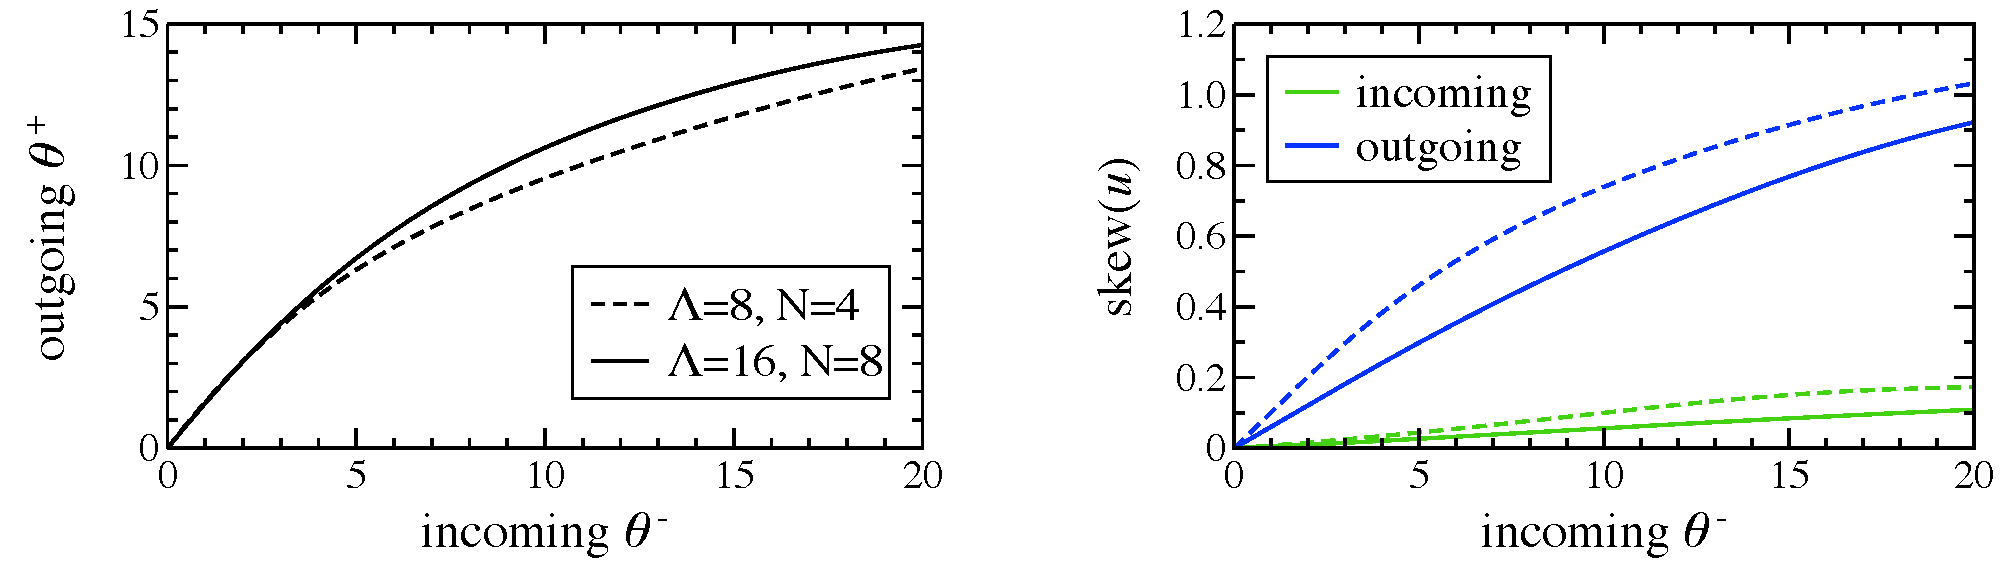
\includegraphics[width = 0.99 \linewidth]{Figs/transfig.pdf}
\caption{
Analysis of the transfer function, $\thdn = \transf \left( \thup \right)$, and calibration of the inverse temperature. (a)--(b) The transfer function for three values of $\Lambda$ with either (a) $\lamfac = 8$ fixed or (b) $\lamfac = \Lambda/2$ scaled. Scaling $\lamfac$ with $\Lambda$ mitigates the sensitivity to $\Lambda$. (c) The incoming and outgoing skewness versus $\thup$ implied by the matching condition. In line with experiments, the skewness is enhanced significantly in the outgoing wave field.
}
\label{transfig}
\end{center}
\end{figure}
 %^^^^^^^^^^^^^^^^^^^^^^^^^^^^^^%
 
	Next, Fig.~\ref{transfig}(b) shows the skewness of the incoming (green) and outgoing (blue) wave fields, as they depend on the incoming inverse temperature $\thup$ for the case $(\Lambda, \lamfac) = (16, 8)$. In line with experimental observations, the incoming skewness is small, while the outgoing wave skewness is much higher. Specifically, to capture the experimentally observed peak skewness range of 0.6-0.9 seen for the larger amplitudes in Fig.~\ref{ExpSpatialStats}(b), requires selecting $\thup$ in the range 10--20.

\subsection{Statistical comparison between theory and experiments}

	We now aim to compare the wave statistics measured in experiments against those that emerge from the TKdV theory. Throughout, we will focus on the representative set of experiments detailed in Table \ref{paramtable}. In these experiments, the peak downstream skewness was measured to be 0.83. We can then use Fig.~\ref{transfig}(c) as a guide to select the appropriate upstream inverse temperature $\thup$. With $(\Lambda, \lamfac) = (16, 8)$ fixed, the figure indicates a value of $\thup = 17$ achieves the desired outgoing skewness. We thus run the deterministic TKdV simulations with model parameters $\Lambda = 16$, $\lamfac = 8$, $\thup = 17$ and with $\epsup$, $\delup$, and $\dratdn$ set to the representative values in Table \ref{paramtable}. We run the simulations to a final dimensionless time of $t_{f} = 10$, with $dt = 5 \times 10^{-4}$ and with $10^3$ trajectories sampled from the upstream Gibbs measure $\Gup$.
	
	We thus run the with these model parameters (and with a sufficiently fine timestep, and number of samples, and to a final dimensionless time of 10).
	
	\vsp{5}
	
	Figure \ref{uhist} shows displacement histograms from these TKdV simulations in comparison to the experiment histograms. The later representative exactly the same data as shown in Fig.~\ref{ExpDiagStats}, only converted to the dimensionless variables. The TKdV simulations do a remarkable job of capturing both the symmetric upstream statistics and the skewed downstream statistics. Amazingly, the simulations reproduce the measured distributions in great detail, both in the shape of the distribution and the scale.
%
This comparison offers convincing evidence that the theory works and the parameters have been matched as well as possible. \nick{Reword and expand}

% Figure
%^^^^^^^^^^^^^^^^^^^^^^^^^^^^^^%
\begin{figure}%[!ht]
\begin{center}
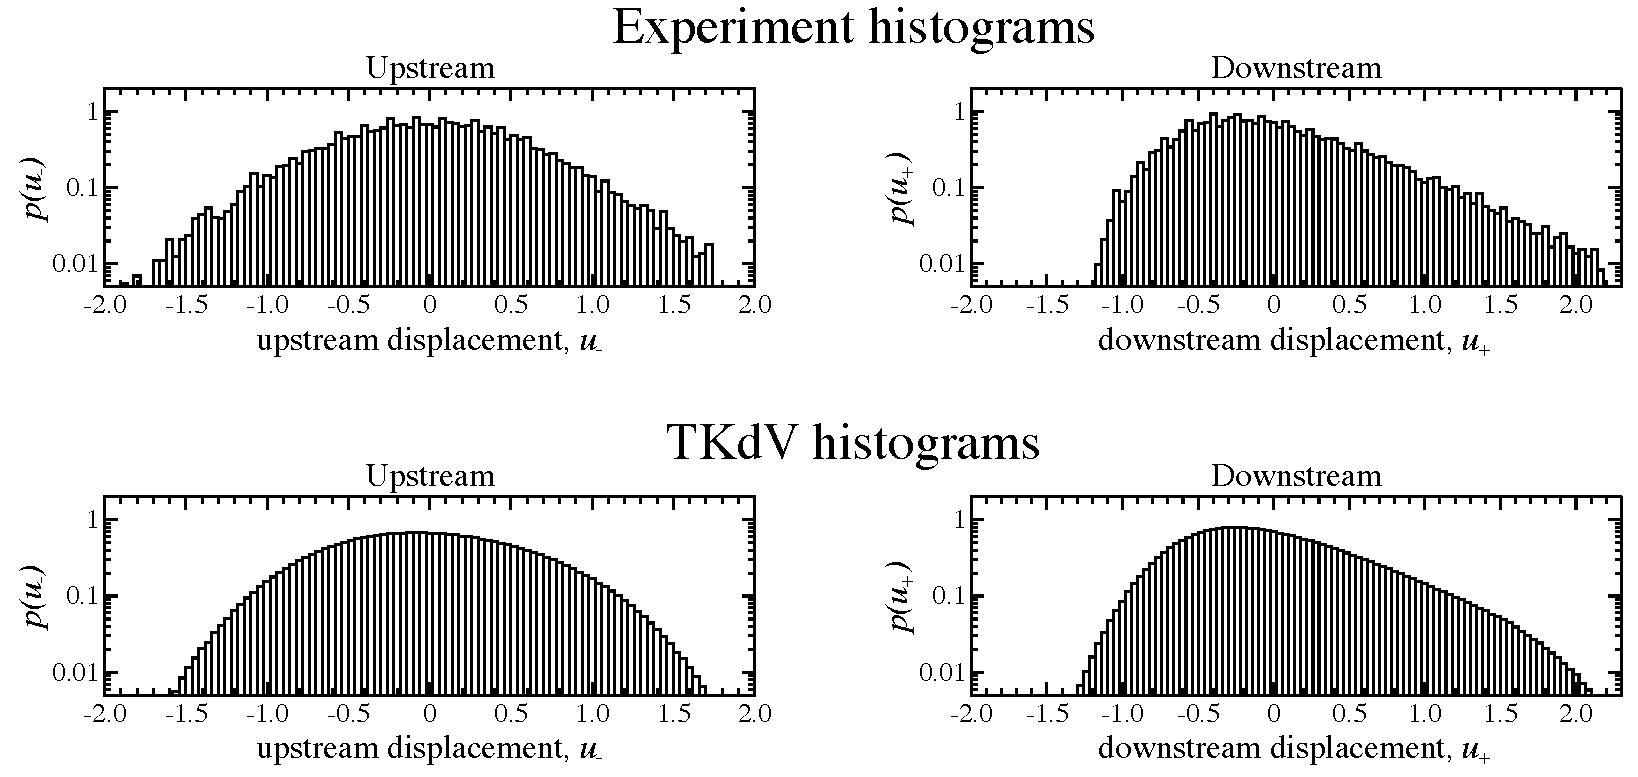
\includegraphics[width = 0.99 \linewidth]{Figs/uhist.pdf}
\caption{ 
Comparison of displacement statistics from experiment and theory. Upon calibrating the inverse temperature $\thup$, the TKdV simulations recover the experimentally measured statistics in remarkable detail. In particular, they exhibit the transition from a nearly symmetric distribution upstream to a highly skewed distribution downstream.
}
\label{uhist}
\end{center}
\end{figure}
 %^^^^^^^^^^^^^^^^^^^^^^^^^^^^^^%
% As of now the simulations use thup=15, thdn=13.

We show histograms of the surface slope in Fig.~\ref{slopehist}, from both the experiments (top) and theory (bottom). The derivative, $\partial \eta / \partial x$, is already a dimensionless quantity with a simple physical interpretation, namely the slope of the free surface, whereas the interpretation of the normalized derivative $\partial u/\partial \tilde{x}$ is tied to the characteristic values $\ampscale$ and $\lengthscale$. 
Therefore, in Fig.~\ref{slopehist}, we convert the theoretical calculated values to physical slope via
\begin{equation}
\pd{\eta}{x} = 2 \pi^{3/2} \frac{\etastd}{\lamupdn} \pd{\uupdn}{\tilde{x}}
%\frac{\ampscale \lamfac}{\lengthscale} \pd{\uupdn}{\tilde{x}}
\end{equation}
In order to map the slope of the wavelength $\lam$ corresponding to $\freqp = 2$ Hz in the experiments onto the dominant spectral mode in the theory, the above conversion has not been corrected with the extra factor of $\lamfac$.

	These slope histograms show intriguing similarities and differences. First, the upstream slope distribution is captured well by the TKdV simulations, both in its nearly symmetric shape and its scale. We note that, while the standard deviation of displacement was input into the TKdV theory, the slope standard deviation was not. Downstream, both the experimental and theoretical slope distributions  spread significantly. Interestingly, in the experiments, it is not the standard deviation of slope that increases significantly upon crossing the depth change ($\std(\eta_x)$ increases from 0.15 to 0.17), but the excess kurtosis that jumps from a value of 0.46 to 3.4. Likewise, in the TKdV theory, $\std(\eta_x)$ grows from 0.13 upstream to 0.33 downstream, and $\kurt(\eta_x)$ grows from -0.04 to 0.50. Thus, the jump in kurtosis, while not as extreme as that measured in experiments, is quite significant in the theory. These elevated levels of kurtosis give the distributions the look of being stretched in the tails and pointy near the centers (especially in the experiments).

	Distinct differences in the shapes of the downstream slope distributions, however, are visible. While the theoretical distributions remain symmetric, the experimental distributions skew towards negative slope. As mentioned earlier, this skewness is consistent with a right-moving wave of steep leading surface (i.e.~negative slope), which is a phenomenon apparently not captured by the TKdV simulations.
Finally, it should be commented that the experimental measurements of slope involve numerical differentiation of the free surface extracted from optical images, which naturally introduces error. Furthermore, high-order statistics, such as kurtosis, can be very sensitive to noise and measurement error. Hence, the experimental statistics of slope, while they are valuable, should be regarded with some level of caution.

% Figure
%^^^^^^^^^^^^^^^^^^^^^^^^^^^^^^%
\begin{figure}%[!ht]
\begin{center}
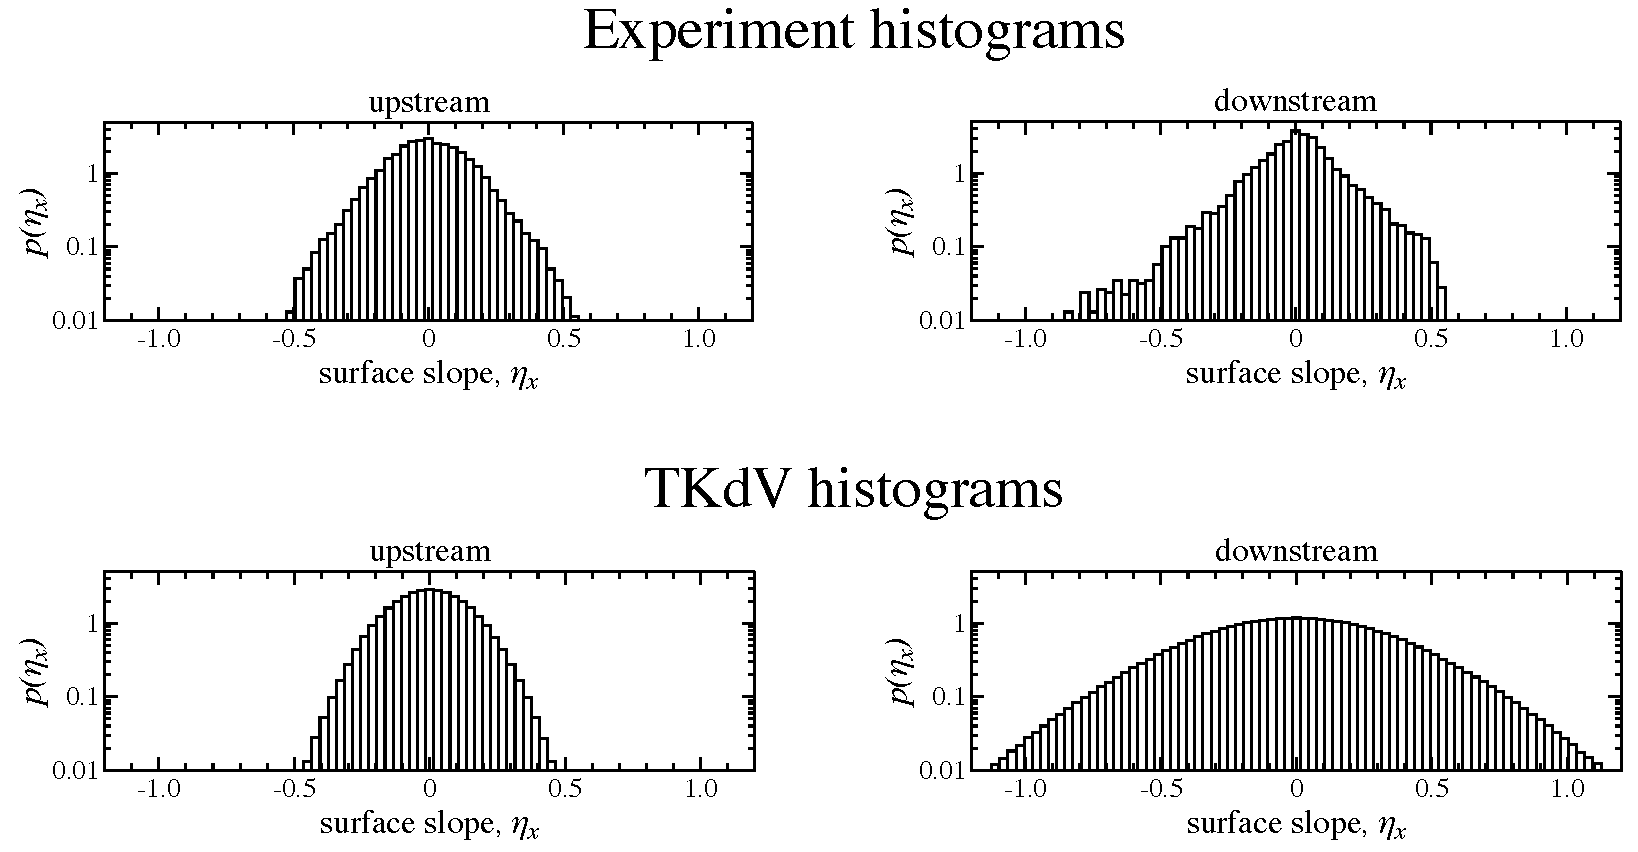
\includegraphics[width = 0.99 \linewidth]{Figs/slopehist.pdf}
\caption{
Comparison of slope statistics. The TKdV simulations show similar slope distributions upstream, but visual distributions in the downstream distributions are visible. While the simulations recover the spread of the downstream slope statistics, they do not capture the asymmetry seen in the experiments.
}
\label{slopehist}
\end{center}
\end{figure}
 %^^^^^^^^^^^^^^^^^^^^^^^^^^^^^^%
% As of now the simulations use thup=15, thdn=13.

\subsection{Wave dynamics}

Next, to complement the statistical comparison, we investigate some individual solution trajectories from the TKdV simulations.

\vsp{5}
We show individual trajectories in the next figure for upstream and downstream. In the upstream flow, due to the coefficients, the nonlinearity is very weak. Hence, wave propagation is dominated by linear dispersion. Indeed, with weak nonlinearity, \eqref{dimlessKdV} is approximated by
\begin{equation}
u_t + C_2 \drat^{1/2} \, u_{xxx} = 0
\qquad \text{for } x \in [-\pi,\pi] \\
\end{equation}
which implies the dispersion relation $\omega_k = -C_2 k^3$ or for phase velocity $c_k = -C_2 k^2$, which implies left-going waves \cite{majdaqi2019}.
% Further details, see page 6 of Majda Qi, J Stat Phys.

% Figure
%^^^^^^^^^^^^^^^^^^^^^^^^^^^^^^%
\begin{figure}%[!ht]
\begin{center}
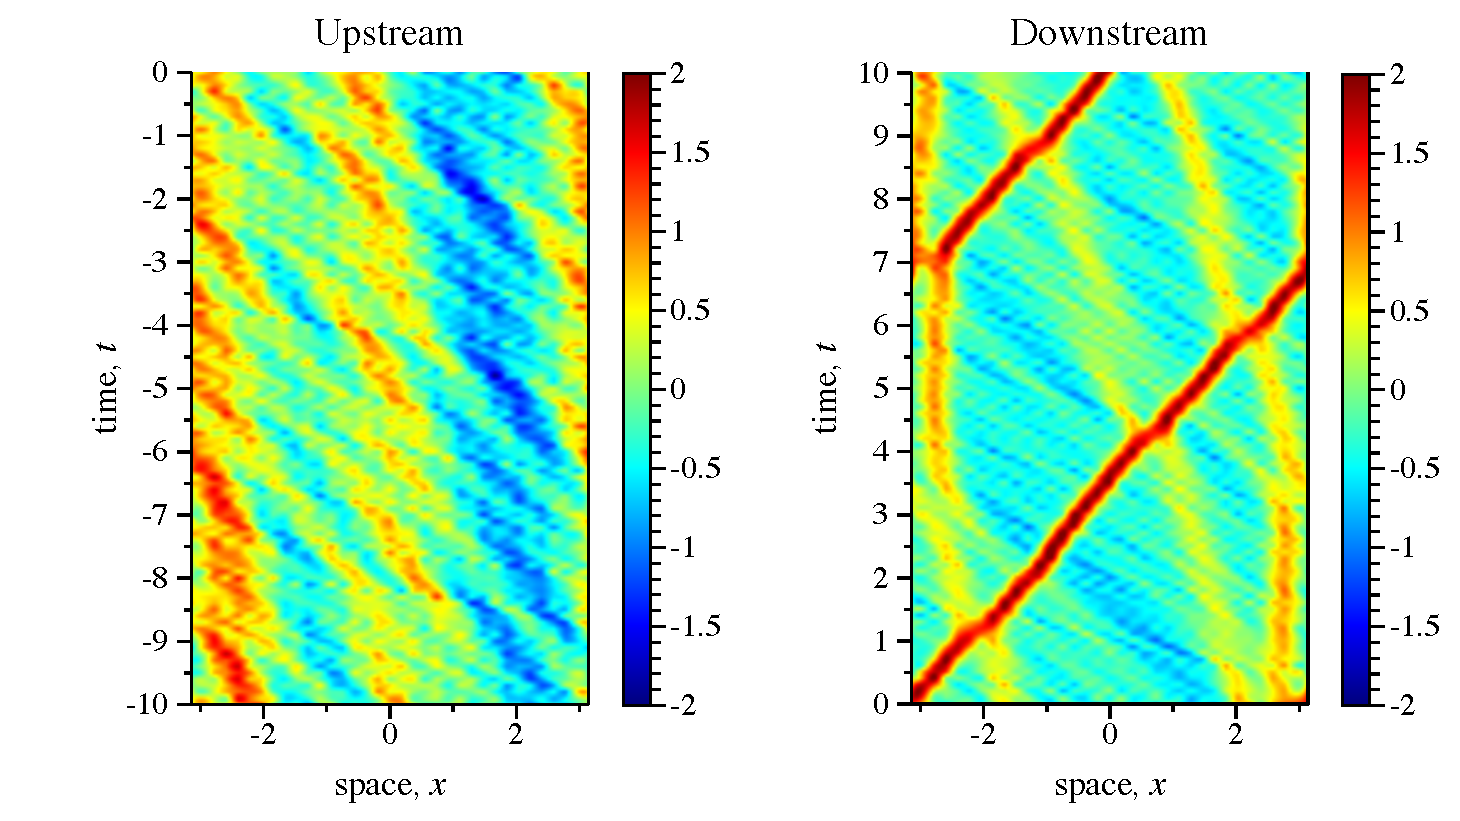
\includegraphics[width = 0.99 \linewidth]{Figs/trajectories.pdf}
\caption{
Sample upstream and downstream solution trajectories from the same ensemble TKdV simulations featured in Figs.~\ref{uhist} and \ref{slopehist}. The upstream solutions exhibit only leftward propagating waves and a high degree of regularity, while the downstream solutions exhibit both left and rightward moving waves along with more intermittency.
}
\label{trajectories}
\end{center}
\end{figure}
 %^^^^^^^^^^^^^^^^^^^^^^^^^^^^^^%

% Figure
%^^^^^^^^^^^^^^^^^^^^^^^^^^^^^^%
\begin{figure}%[!ht]
\begin{center}
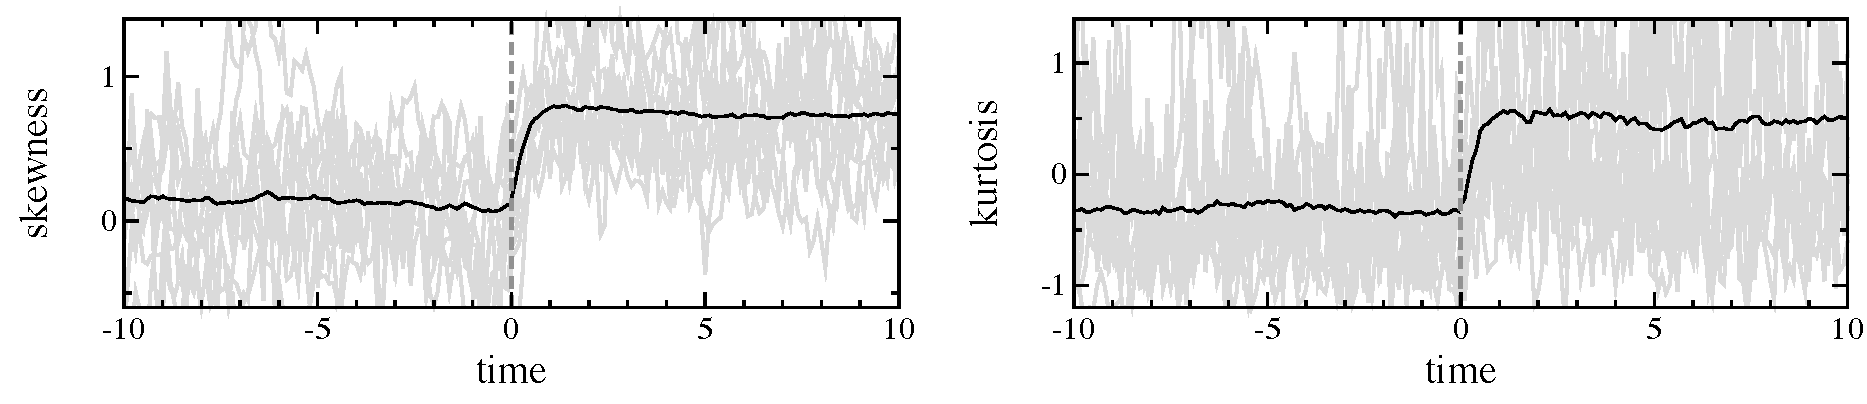
\includegraphics[width = 0.99 \linewidth]{Figs/skew-kurt.pdf}
\caption{
Skewness and kurtosis in DNS}
\label{skew-kurt}
\end{center}
\end{figure}
 %^^^^^^^^^^^^^^^^^^^^^^^^^^^^^^%
 
 
\vsp{5}
%----------------------------------------------------------------------------%
% Skewness formula
%----------------------------------------------------------------------------%
\subsection{Explicit formula for outgoing skewness}
We now examine an explicit formula for the outgoing skewness as originally founded in \cite{majda2019}.
An experimental observation is that the incoming skewness is small, $\meanup{H_3} \approx 0$. Inserting this approximation into the statistical matching condition \eqref{statmatch} and simplifying gives
\begin{equation}
\label{H3H2}
\frac{\meandn{\Hthree^+}} {\meandn{\Htwo^+} - \meanup{\Htwo^+}} = \frac{C_2}{C_3} \dratdn^2
\end{equation}
%where $\Delta \mean{H_2} =  \meandn{H_2} - \meanup{H_2}$  indicates the difference between the upstream and downstream values.
To convert to dimensional, i.e.~experimental, values we first note that
\begin{align}
\mean{\Hthree^+} = \frac{\pi}{3} \mean{u^3} = 
\frac{1}{3} \pi^{-1/2} \frac{\mean{\eta^3}}{\etastd^3} = \frac{1}{3} \pi^{-1/2} \skw(\eta)
\end{align}
Second, to convert the downstream surface slope, we note
\begin{align}
\pd{u}{\tilde{x}} = \frac{\lamfac \lamdn}{\pi^{3/2} \etastd} \pd{\eta}{\xi}
\end{align}
where slope with respect to $\xi$ is the same as with respect to dimensional $x$.
Note: I believe it is important here to use $\lamdn$ in reverting to dimensional variables since we are matching $\Hdn$.
Hence, we have
\begin{align}
&\mean{\Htwo^+} = \pi \mean{ \left( \pd{u}{\tilde{x}} \right)^2} = 
\left( \frac{\lamfac \lamdn}{\pi \etastd} \right)^2 \var(\eta_x)
\end{align}
%
Then algebra gives
\begin{equation}
\frac{\meandn{\Hthree}} {\meandn{\Htwo} - \meanup{\Htwo}} = 
\frac{\pi^{3/2} \, \etastd^2} {3 \lamfac^2 \lamdn^2} 
\left( \frac{\skwdn(\eta)} { \vardn(\eta_x) - \varup(\eta_x)} \right)
\end{equation}
Also we have the simplification
\begin{equation}
\frac{C_2}{C_3} = \frac{\pi^{3/2} \delup^2}{9 \lamfac^2 \epsup}
\end{equation}
Hence, \eqref{H3H2} gives the remarkably explicit formula
\begin{equation}
\frac{\skwdn(\eta)} {\vardn(\eta_x) - \varup(\eta_x)} = \frac{1}{3} \epsup^{-3} \dratdn^3 =
\frac{1}{3} \left( \frac{\ddn}{\etastd} \right)^3
\end{equation}
In particular, the ratio on the left, which can be measured in the experiments, is predicted to scale as the inverse cube of the wave amplitude and as the square of the depth ratio.
% Note: previously I had D^2 on the RHS. The power of 3 comes from using lamdn consistently in the nondimensionalization.






\vsp{10}
%----------------------------------------------------------%
% Direct numerical simulations
%----------------------------------------------------------%
\section{Direct numerical simulations}

\section{Sampling Algorithms}
%\subsection{Naive acceptance-rejection algorithm}
%\subsection{Markov-chain Monte Carlo}
%\subsection{Improved acceptance-rejection algorithm}


%----------------------------------------------------------%
% Comparison with experiments
%----------------------------------------------------------%
\section{Comparison with experiments}

% Figure
%^^^^^^^^^^^^^^^^^^^^^^^^^^^^^^%
\begin{figure}%[!ht]
\begin{center}
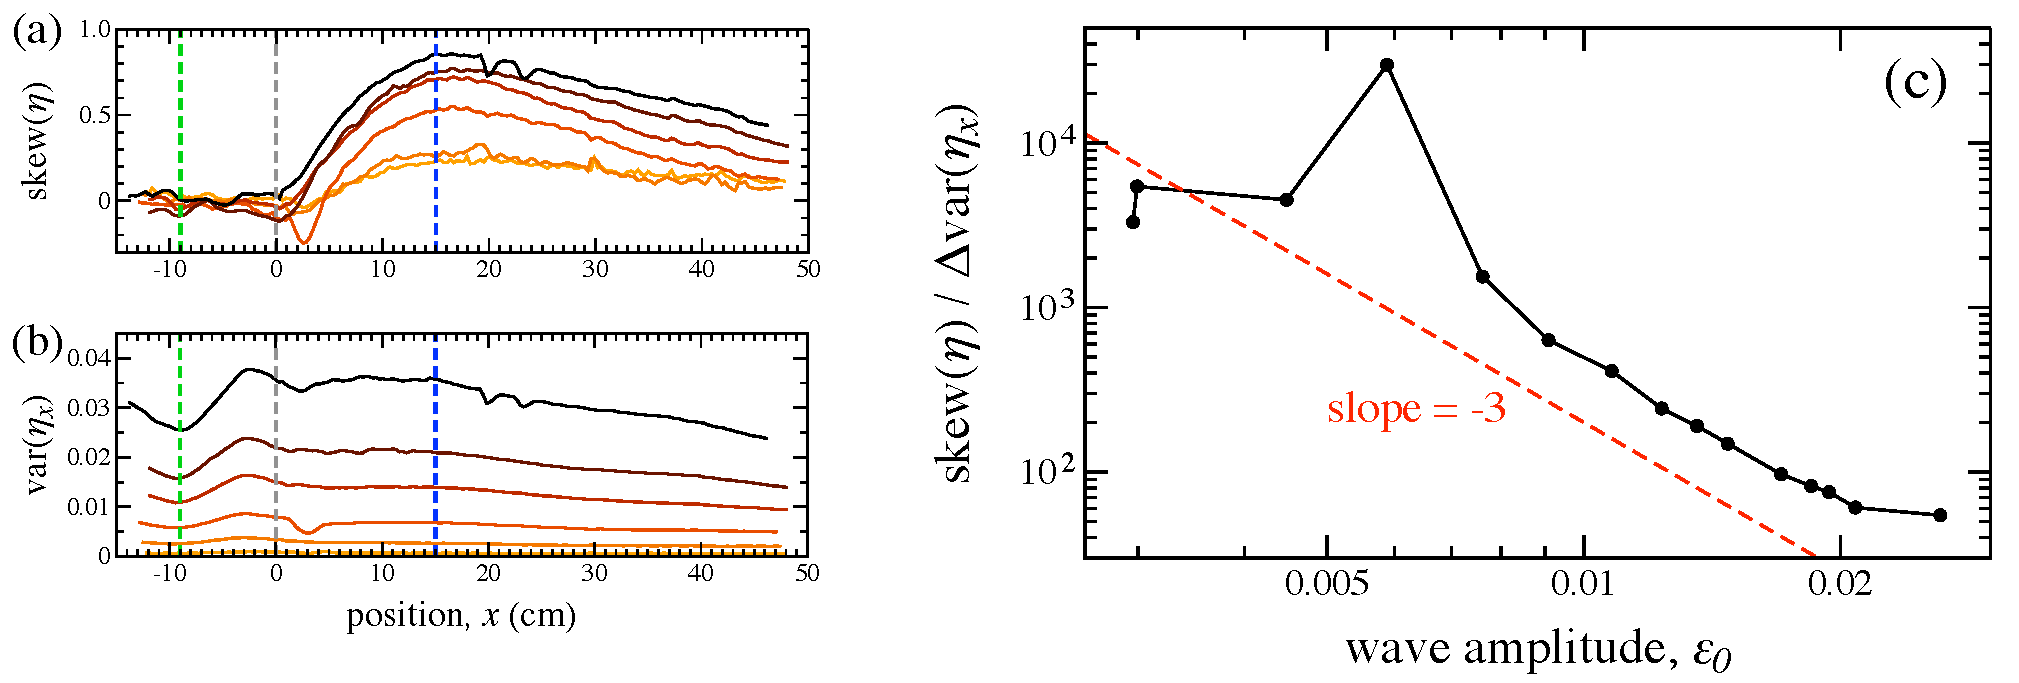
\includegraphics[width = 0.99 \linewidth]{Figs/SkewRat.pdf}
\caption{
Relationship predicted by the theory and confirmed by experiments.
}
\label{AAA}
\end{center}
\end{figure}
 %^^^^^^^^^^^^^^^^^^^^^^^^^^^^^^%
 %New experimental measurements guided by theory

\section*{Acknowledgements}
CTB acknowledges support from the IDEA grant at Florida State University, as well as from the Geophysical Fluid Dynamics Institute. 
MNJM acknowledges support from the Simons Foundation, award 524259. 

\bibliographystyle{plain}
\bibliography{wavesbib}

\end{document}
